% !TEX TS-program = pdflatex
% !TEX root = ../LightMicroRep.tex

%************************************************
\chapter{Fluorescence Recovery After Photobleaching}
\label{chp:FRAP}
%************************************************
%\numberwithin{figure}{section}
%----------------------------------------------------------------------------------------
%	INTRODUCTION
%----------------------------------------------------------------------------------------

\section{Introduction}

\paragraph{Aim} To investigate the dynamics of two different proteins (NE81 and Erg24) after photobleaching.
\\

In this experiment, Fluorescence Recovery After Photobleaching (FRAP) method is utilized to investigate the dynamics of proteins in a living cell. 
Photobleaching refers to the fact that fluorescently tagged proteins are bleached by high intensity laser on certain parts/area of the cell, all the while the sample are continuously imaged by fluorescence imaging. 
Observation on this bleached area would result in whether or not fluorescence on this area recovers over time.

Two proteins from two different cells are tagged by GFP, namely NE81 in \textit{Dictyostelium discoideum} and Erg24 in yeast cells. 
NE81 is a lamin-like protein that associates with the inner nuclear envelope of Dictyostelium cells and plays a role in the formation of a nuclear lamina \cite{Krueger2012}. 
Erg24 is an enzyme that is involved in ergosterol/sterol biosynthesis \cite{UniprotErg24}. It is a membrane protein mostly found in yeast, but also exist in other organism as well \cite{Batsios2019}.

%----------------------------------------------------------------------------------------
%	METHODS
%----------------------------------------------------------------------------------------

\section{Methods}
FRAP measurements was conducted to two proteins (NE81 and Erg24, both tagged with GFP) in living cells. 
Experiment was conducted twice for each protein, yielding in two image series (movies) of each protein.

Data sampling of selected cells on the image series over time was done through imageJ (Fiji) and saved as csv files. 
These data are then combined (for both image series of one protein) and processed in a script written in \faRProject~(available publicly on \href{https://gitup.uni-potsdam.de/showard/lightmicroscopy}{\faGitlab~gitUP}, or by request).

The sampling procedure involves in measuring on a certain area (RoI - Region of Interest) the fluorescence intensity of: 
\begin{itemize}
\item photobleached cells (two frames pre-bleaching and afterwards until the last frame)
\item several unbleached cells (all frames)
\item the background (all frames)
\end{itemize}

Calculation and plotting procedure involves several steps:
\begin{enumerate}
\item Averaging the background signal across all frames
\item Substracting the fluorescence signal of the sampled cells by the background
\item Normalize the fluorescence signal of unbleached cells by the average measurements of the first two frames
\item Plot the unbleached measurements to obtain the slope for corrections
\item Normalize the fluorescence signal of photobleached proteins by the average measurement of the two frames pre-bleaching
\item Apply correction that is obtained by the slope of unbleached cells to the photobleached cells measurements
\item Average all corrected measurements of photobleached cells and plot against time
\end{enumerate}
%----------------------------------------------------------------------------------------
%	RESULTS AND DISCUSSION
%----------------------------------------------------------------------------------------
\section{Results and Discussion}

As can be seen on the resulting FRAP plots (Fig.~\ref{fig:FRAPres}), the two proteins behave distinctly. 
It is evident that the measurement of NE81 does not recover the fluorescence over time, unlike the fluorescence of Erg24 that increases again. 

Scrutinizing the plot in more detail, it can be seen in Fig.~\ref{NE81} that there are rather large errors of the fluorescent intensity measurement at certain time points. 
This wide error is due to the difficulty encountered during sampling using imageJ in which it is quite tricky to follow the RoI (Region of Interest) of the cells all across the time points of the image series, because the cells are moving everywhere along the 2D axes and also twisting around. 
And the fact that cells of this protein samples are quite small does not help the (manual) sampling using imageJ at all.
This difficulty results in some outlying sampling data which widens the error bars. 
A closer inspection on the sampling data (shown by the green boxes in Fig.~\ref{NE81}) shows that a certain number of sampling could be done in a more accurate manner. 
However since the outlying sampling data were sparse and occured on different sampled cells, taking into account that the final data would be constituted by the combined result of many sampled cells, no attempt or justification were made to neither remove any outlying data points nor resampling the image series. 
As can be demonstrated, all the calculation procedures were applied successfully, despite the relatively wide error bars on certain time points. 

The resulting plot of NE81 shows that no recovery can be observed after photobleaching. 
This phenomenon is captured by the slope of the trendline ($-0.00028$) that indicates that the fluorescence signal stagnates, or even decreasing over time.
 This decrease can be attributed to natural occurences that make fluorescence intensity decreases over time, even without bleaching, such as: exposure to light, molecules being destroyed, etc. 
 The stagnation means that once the photobleaching occured, NE81 proteins on the area get destroyed, but diffusion or transport of NE81 proteins from other parts of the cell does not occur. 
 Literature suggest that the immobility of NE81 indicates that the cells in the sample are existing in the interphase, because NE81 are mobile during mitosis \cite{Krueger2012}.

\begin{figure}[h!]
\centering
\subfloat[NE81\label{NE81}]{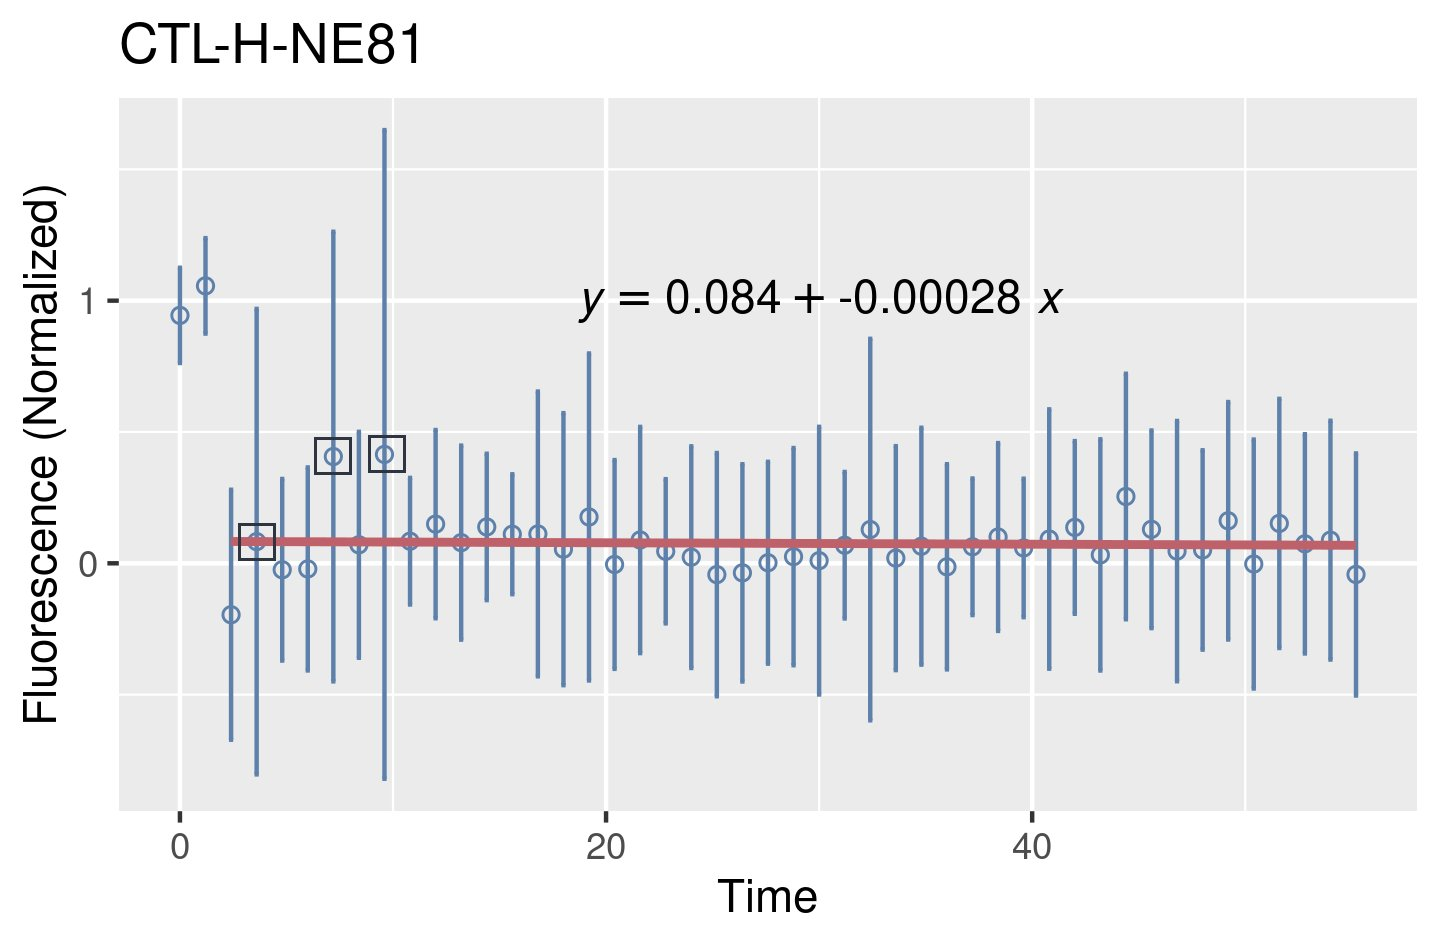
\includegraphics[width=.85\columnwidth]{Exp_10_FRAP/Figures/CTL-H-NE81BGsd_nor2}}\\
\subfloat[Erg24\label{Erg24}]{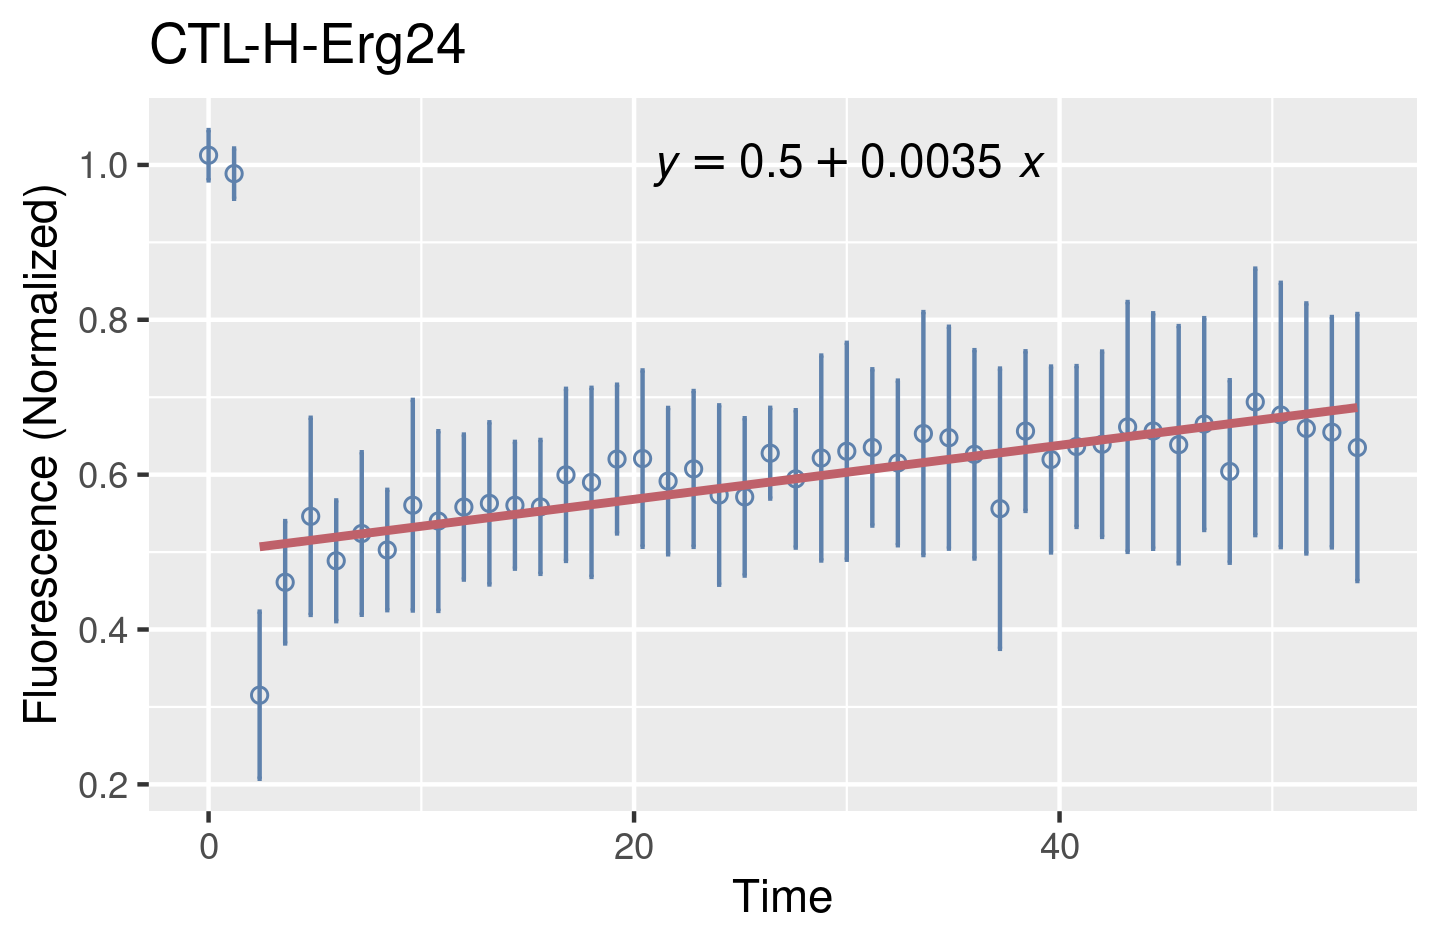
\includegraphics[width=.85\columnwidth]{Exp_10_FRAP/Figures/CTL-H-Erg24BGsd_nor2}} \\
\caption[FRAPres]{FRAP plot of the proteins NE81 (\textbf{A}) and Erg24 (\textbf{B}). 
Trendline is made from the datapoints, excluding the first two unbleached measurements. 
The slope (m) of the trendline for NE81 is $-0.00028$ and for Erg24 is $0.0035$. 
Boxes on \textbf{A} indicates the inspected sampling points.} 
\label{fig:FRAPres}
\end{figure}

The plot of protein Erg24 (Fig.~\ref{Erg24}) shows a different dynamic behaviour. 
Unlike NE81, the fluorescence signal increases over time, indicated by the slope of the tredline ($0.0035$). 
This increase is due to the diffusion or transport of proteins from other parts of the cells. The recovery of the fluorescence signal during the experiment does not return to the original intensity, probably due to the time frame of the experiment. 
Nevertheless, the movement of Erg24 proteins in photobleached cells is corroborated by literature as well \cite{Batsios2019}.

The difficulty encountered during the sampling of NE81 proteins for the most part did not occur for this Erg24 protein, this is mostly due to the fact that the cells for this specimen are larger, and hence the bleached area can be tracked more accurately and also precaution has been taken after the sampling of NE81. 
This is reflected by the error bars of the measurement on each time point that do not indicate any significantly outlying sampling data.

The slope shown on the fluorescence recovery plots of both proteins, along with the trendline, are merely shown to help capture the tendency of how the fluorescence signal develops after photobleaching and does not in any way speculate about the linearity of the datapoints. 
As indicated by the plot of Erg24 and the common fluorescence recovery curves, it is possibly not linear at all. 
Curve fitting to obtain the half-life of recovery ($t_{1/2}$) was not attempted because access to the software package of the microscope is limited at the point of writing this report~\cite{LectLCI}. 
 
In conclusion, it can be seen that the mobility of protein NE81 in \textit{Dictyostelium discoideum} and Erg24 in yeast cells after photobleaching differs significantly, in which NE81 does not recover the fluorescence intensity signal and hence does not exhibit any movement, on the contrary, Erg24 recovers its fluorescence intensity signal in the area that is photobleached indicating that there is movement of the protein toward the photobleached area from other parts of the cell.


%----------------------------------------------------------------------------------------
%	BIBLIOGRAPHY
%----------------------------------------------------------------------------------------

\renewcommand{\refname}{\spacedlowsmallcaps{References}} % For modifying the bibliography heading

%\bibliographystyle{unsrt}

%\bibliography{sample.bib} % The file containing the bibliography

%----------------------------------------------------------------------------------------
